\documentclass[tikz,border=4pt]{standalone}
\usepackage{pgfplots}
\pgfplotsset{compat=1.18}
\begin{document}
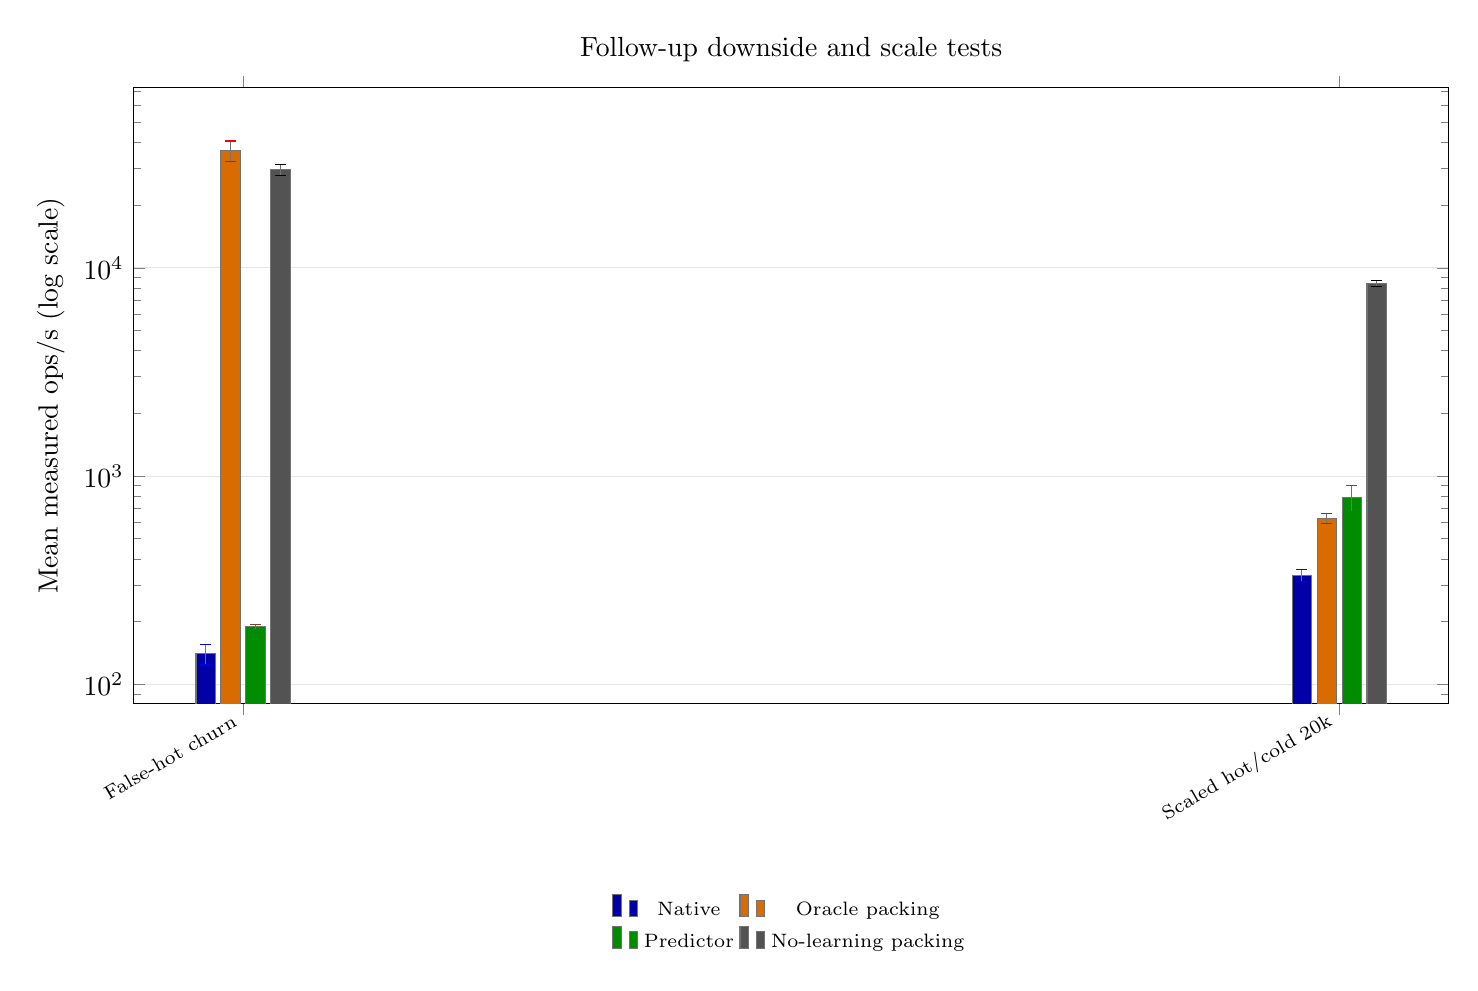
\begin{tikzpicture}
\begin{axis}[
  title={Follow-up downside and scale tests},
  width=7.2in,
  height=3.7in,
  ybar,
  bar width=7pt,
  enlarge x limits=0.10,
  ylabel={Mean measured ops/s (log scale)},
  ymin=81.0618,
  ymax=73092.9,
  ymode=log,
  xtick={0,1},
  xticklabels={False-hot churn,Scaled hot/cold 20k},
  x tick label style={rotate=30,anchor=east,font=\scriptsize},
  ymajorgrids=true,
  grid style={draw=gray!20},
  legend style={at={(0.5,-0.30)},anchor=north,legend columns=2,font=\scriptsize,draw=none},
  error bars/y dir=both,
  error bars/y explicit,
]
\addplot+[fill=blue!65!black,draw=black!55,bar shift=-13.5pt]
coordinates {
  (0,140.339) +- (0,15.6289)
  (1,334.599) +- (0,21.3189)
};
\addlegendentry{Native}
\addplot+[fill=orange!85!black,draw=black!55,bar shift=-4.5pt]
coordinates {
  (0,36537.8) +- (0,4069.38)
  (1,626.403) +- (0,36.0175)
};
\addlegendentry{Oracle packing}
\addplot+[fill=green!55!black,draw=black!55,bar shift=4.5pt]
coordinates {
  (0,188.957) +- (0,5.26044)
  (1,791.915) +- (0,113.533)
};
\addlegendentry{Predictor}
\addplot+[fill=gray!65!black,draw=black!55,bar shift=13.5pt]
coordinates {
  (0,29632.5) +- (0,1765.3)
  (1,8389.15) +- (0,292.441)
};
\addlegendentry{No-learning packing}
\end{axis}
\end{tikzpicture}
\end{document}